\FloatBarrier
Before the idea of behavioral cloning can be tackled, which got described in section \ref{sec::51_bc}, one needs to meet the prerequisites, that is one must calibrate the camera, and tune the depth map extraction parameters, which will be done within this chapter in sections \ref{sec::10_cc}, and \ref{sec::102_dp}, respectively.
\section{Camera Calibration}
\label{sec::10_cc}
As described in section \ref{sec::3_ip}, for the stereo block matching algorithm to work properly (equation \ref{eq::31_sad}), it is required to calibrate the cameras. This is shortly verified in figure \ref{fig::101_no_calib}, where a depth map got extracted from the uncalibrated stereo camera pair.
\begin{figure}[h!]
	\centering
	\subcaptionbox{Left disparity map.}%
	[.4\linewidth]{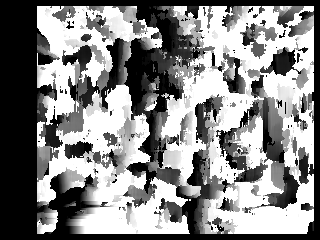
\includegraphics[scale=.3]{chapters/10_image_processing_experiments/img/disp_no_calib.png}}
	\subcaptionbox{Confidence weighted least squares filtered disparity map.}%
	[.4\linewidth]{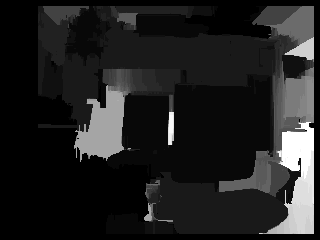
\includegraphics[scale=.3]{chapters/10_image_processing_experiments/img/wls_no_calib.png}}
	\caption{Depth map extraction without calibration. The parameters were set as follows to $N=13$, $D=32$, $\sigma = 1$, and $\lambda=10^4$.}
	\label{fig::101_no_calib}
\end{figure}
For the calibration a chess-board calibration pattern was chosen, see figure \ref{fig::101_calib}. The used calibration pattern has width of $W=8$, and a height of $H=6$, where each square has a size of $a=22.5\,\text{mm}$ (equation \ref{eq::32_square_size}). A total of $N=60$ images of the calibration pattern was taken for varying orientations and translations with respect to the camera, which results in a total of $W\times H\times N = 2880$ points for the calibration. 
\begin{figure}[h!]
	\centering
	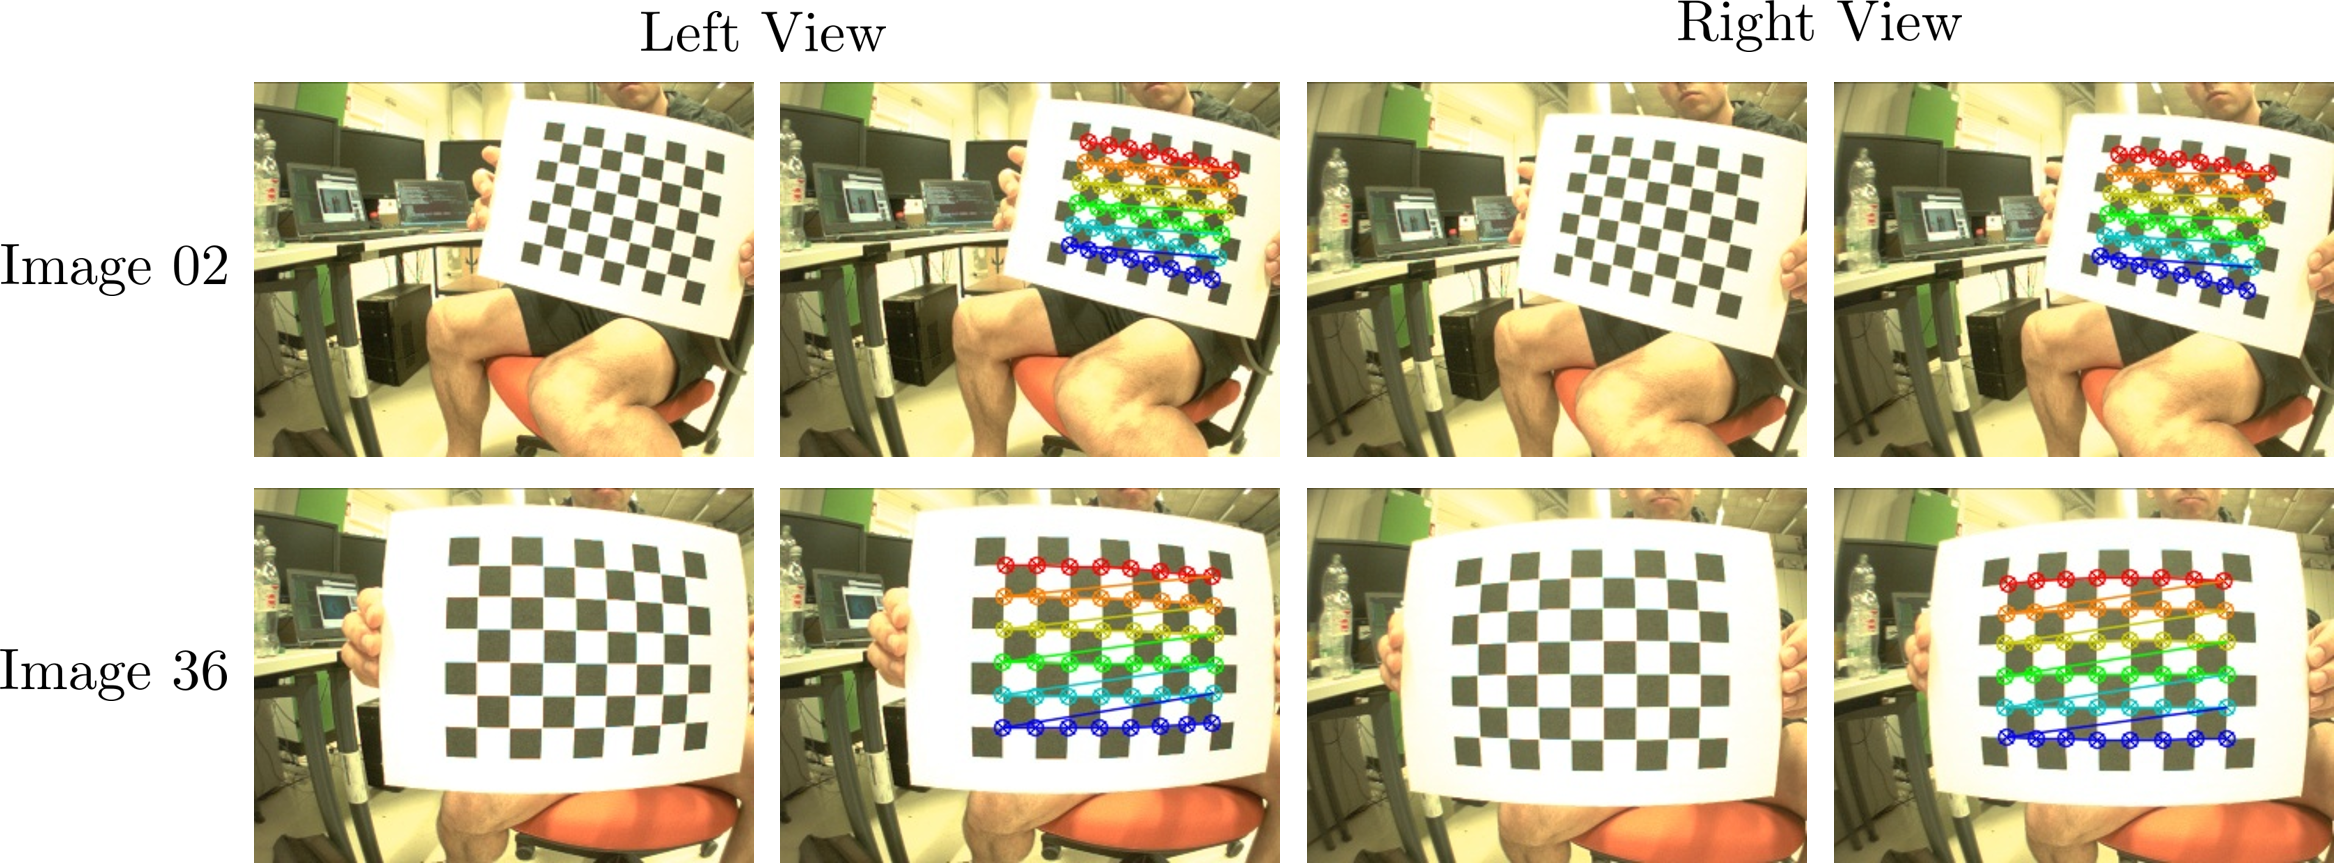
\includegraphics[scale=.28]{chapters/10_image_processing_experiments/img/calib.png}
	\caption{Exemplary left and right camera views of the calibration pattern as acquired during the calibration process. The colorful points indicate the detected corners in the image plane. Refer to section \ref{sec::32_cc} for the theory.}
	\label{fig::101_calib}
\end{figure}
The resulting mean squared re-projection error $\Delta \bar{x} = 1/(WHN)\sum_0^{WHN} \Delta x$ (equation \ref{eq::32_reprojection}), is $\Delta \bar{x}_l = 0.26\, \text{pixel}$, and $\Delta \bar{x}_r = 0.25\,\text{pixel}$, for the left, and the right camera, respectively. According to equations \ref{eq::32_focal_intrinsics}, \ref{eq::32_x_dist}, and \ref{eq::32_y_dist}, the camera's intrinsic parameters were, therefore, determined as listed in table \ref{tab::101_intrinsics}.
\begin{table}
	\centering
	\caption{Intrinsic parameters of single cameras. These parameters can be found as YAML file on GitHub (\href{https://github.com/mhubii/nmpc_pattern_generator/tree/master/libs/io_module}{\underline{link}}).\label{tab::101_intrinsics}}
	\begin{tabular}{lll}
		Intrinsic Parameter & Left Camera & Right Camera\\
		\hline
		$f_x\,[\text{pixel}/\text{mm}]$ & $\quad2.36\cdot10^2$ & $\quad2.32\cdot10^2$ \\
		$f_y\,[\text{pixel}/\text{mm}]$ & $\quad2.37\cdot10^2$ & $\quad2.32\cdot10^2$ \\
		$c_x\,[\text{pixel}]$ & $\quad1.63\cdot10^2$ & $\quad1.86\cdot10^2$ \\
		$c_y\,[\text{pixel}]$ & $\quad1.11\cdot10^2$ & $\quad1.30\cdot10^2$ \\
		$k_1\,[1/\text{pixel}^2]$ & $-4.54\cdot10^{-1}$ & $-4.58\cdot10^{-1}$ \\
		$k_2\,[1/\text{pixel}^4]$ & $\quad2.90\cdot10^{-1}$  & $\quad3.18\cdot10^{-1}$  \\
		$k_3\,[1/\text{pixel}^6]$ & $-1.21\cdot10^{-1}$ & $-1.48\cdot10^{-1}$ \\
		$p_1\,[1/\text{pixel}]$ & $-2.73\cdot10^{-3}$ & $\quad3.02\cdot10^{-4}$  \\
		$p_2\,[1/\text{pixel}]$ & $\quad2.16\cdot10^{-4}$  & $\quad7.63\cdot10^{-4}$		
	\end{tabular}
\end{table}
Then given the calibration of each single camera, the rectification transforms $\bm{R}_i$, and the projection matrices $\bm{P}_i$ in the rectified coordinate system, was determined for each camera, all of which can be found in table \ref{tab::101_extrinsics}.
\begin{table}
	\centering
	\caption{Rectification transforms $\bm{R}_i$, and projection matrices $\bm{P}_i$, for the left, and the right camera, respectively. These parameters can be found as YAML file on GitHub (\href{https://github.com/mhubii/nmpc_pattern_generator/blob/master/libs/io_module/cam_stereo.yaml}{\underline{link}}). \label{tab::101_extrinsics}}
	\begin{tabular}{lll}
		Camera & Extrinsic Parameter & \\ 
		\hline
		&& \\
		\multirow{5}{*}{Left} & $\bm{R}\,[\text{a.u.}]$              & $\begin{pmatrix}
		\quad9.93\cdot10^{-1} & -2.65\cdot10^{-3}     & \quad1.14\cdot10^{-1} \\ 
		\quad5.41\cdot10^{-1} & \quad1.00\cdot10^{0}  & -2.39\cdot10^{-2} \\
		-1.14\cdot10^{-1}     & \quad2.43\cdot10^{-2} & \quad9.93\cdot10^{-1}
		\end{pmatrix}$ \\&&\\
		& $\bm{P}\,[\text{pixel}/\text{mm}]$              & $\begin{pmatrix}
		2.34\cdot10^{2} & 0.00     & 1.88\cdot10^{2} & 0.00\,\text{mm} \\ 
		0.00 & 2.34\cdot10^{2}  & 4.87\cdot10^{1} & 0.00\,\text{mm} \\
		0.00    & 0.00 & 1.00 & 0.00\,\text{mm}
		\end{pmatrix}$ \\
		&&\\
		\multirow{5}{*}{Right} & $\bm{R}\,[\text{a.u.}]$              & $\begin{pmatrix}
		\quad9.95\cdot10^{-1} & -2.30\cdot10^{-2}     & \quad9.93\cdot10^{-2} \\ 
		\quad2.07\cdot10^{-2} & \quad1.00\cdot10^{0}  & \quad2.38\cdot10^{-2} \\
		-9.98\cdot10^{-2}     & -2.16\cdot10^{-2} & \quad9.95\cdot10^{-1}
		\end{pmatrix}$ \\&&\\
		& $\bm{P}\,[\text{pixel}/\text{mm}]$              & $\begin{pmatrix}
		2.34\cdot10^{2} & 0.00     & 1.88\cdot10^{2} & -1.60\cdot10^1\,\text{mm} \\ 
		0.00 & 2.34\cdot10^{2}  & 4.88\cdot10^{1} & 0.00\,\text{mm} \\
		0.00    & 0.00 & 1.00 & 0.00\,\text{mm}
		\end{pmatrix}$ \\
	\end{tabular}
\end{table}
Exemplary rectified images, which rely on the matrices of table \ref{tab::101_extrinsics}, are shown in figure \ref{fig::101_rect} (a). Since there is a slight rotation of the calibration pattern, it is not obvious that the images got rectified well. Therefore, the same images are shown in figure \ref{fig::101_rect} (b), but slightly rotated such that the calibration pattern aligns horizontally. The blue line therein indicates that in contrast to the original image, straight lines now appear straight across both images, which is crucial for the block matching algorithm in the next section - Depth Map Parameter Tuning.
\begin{figure}[h!]
	\centering
	\subcaptionbox{Rectified images.}%
	[.4\linewidth]{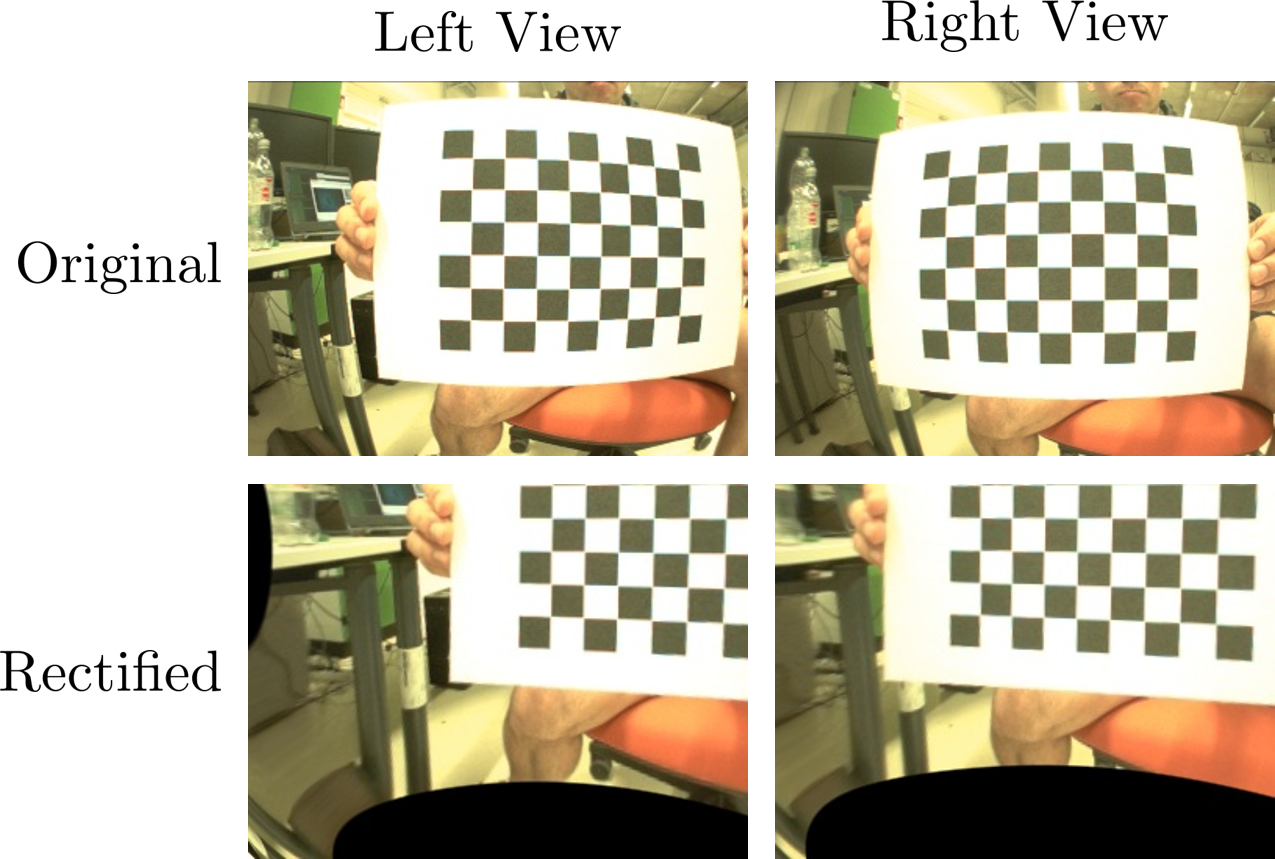
\includegraphics[scale=.25]{chapters/10_image_processing_experiments/img/rect.png}}
	\subcaptionbox{Rotated rectified images.}%
	[.4\linewidth]{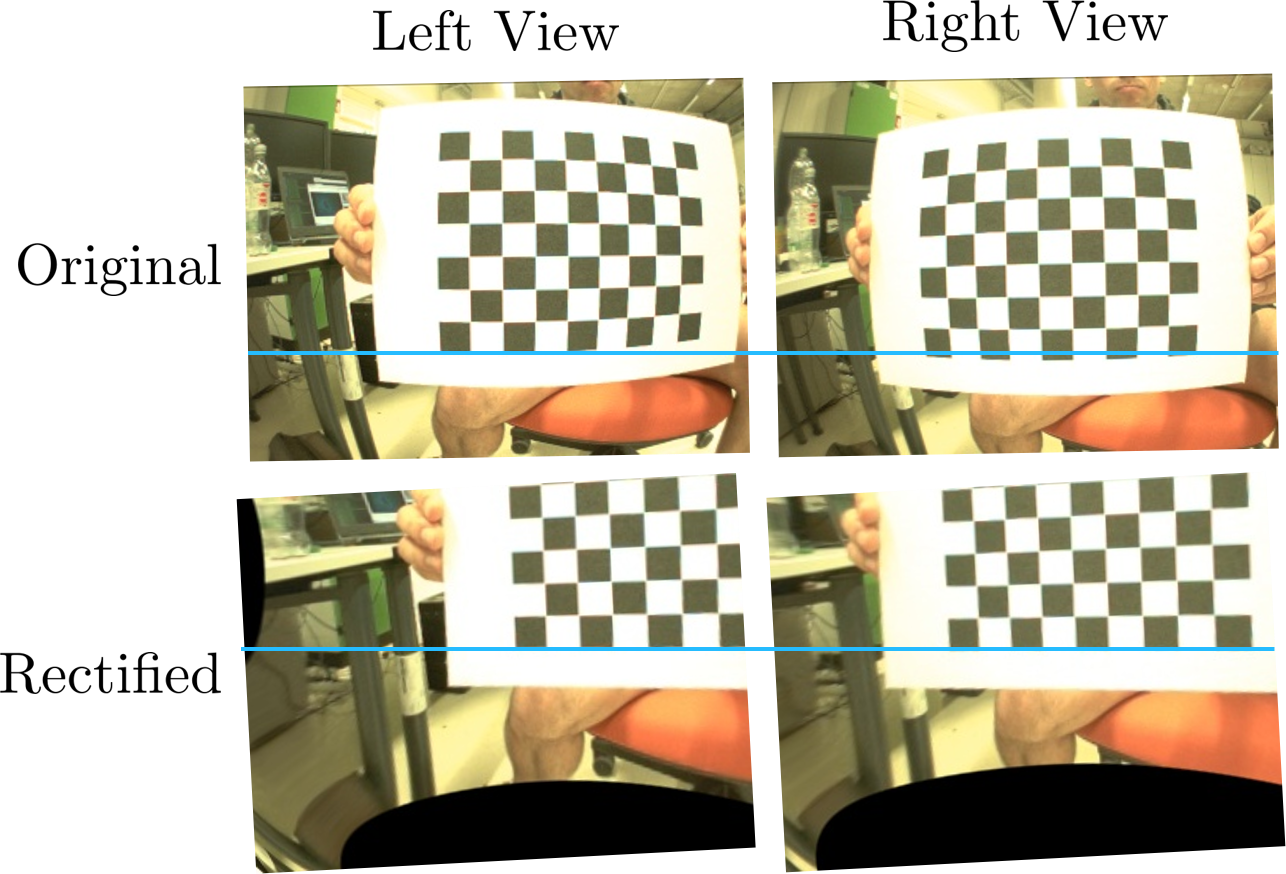
\includegraphics[scale=.25]{chapters/10_image_processing_experiments/img/rect_line.png}}
	\caption{Rectified and original view of the stereo camera. Refer to section \ref{sec::32_cc} for the theory.}
	\label{fig::101_rect}
\end{figure}
\FloatBarrier
\section{Depth Map Parameter Tuning}
\label{sec::102_dp}
Within this section, the effects of all tuneable parameters on the depth map generation are explored. Therefore, a simple experimental setup is used. Within the setup, Heicub points its stereo camera towards three chairs that are located at a distance of $1\,\text{m}$ towards each other, and towards the cameras, so to cover close, medium, and far distances. The consecutive chairs are slightly shifted, in order to enable the simultaneous observation of all of them. The rectified view of the environment is shown in figure \ref{fig::102_wls_rgb}.
\begin{figure}[h!]
	\centering
	\subcaptionbox{Left camera's view.}%
	[.4\linewidth]{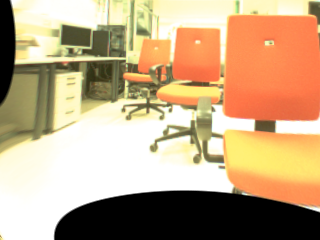
\includegraphics[scale=.3]{chapters/10_image_processing_experiments/img/l_rgb.png}}
	\subcaptionbox{Right camera's view.}%
	[.4\linewidth]{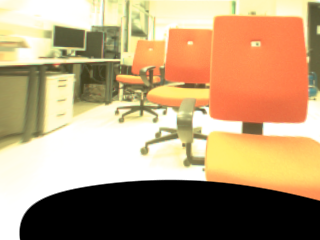
\includegraphics[scale=.3]{chapters/10_image_processing_experiments/img/r_rgb.png}}
	\caption{Heicub's perspective of the scene for the depth map parameter tuning.}
	\label{fig::102_wls_rgb}
\end{figure}
The depth map extraction, which utilizes the rectified images, depends on a stereo block matching algorithm that was explained in section \ref{sec::3_ip}. It mainly depends on the window size and the number of disparities for the sum of absolute difference computation. The influence of those two parameters was evaluated in a grid search fashion in figure \ref{fig::102_disp} (a). It is apparent that the change in the number of disparities has close to no influence onto the depth map quality, while it removes plenty of useful information from the left-hand side of images. The same holds for the window size, except that it removes some noise from the depth maps.
\begin{figure}[h!]
	\centering
	\subcaptionbox{Left disparity. Please refer to figure \ref{fig::31_left_disparity_map} and equation \ref{eq::31_sad} for the theory.}%
	[.45\linewidth]{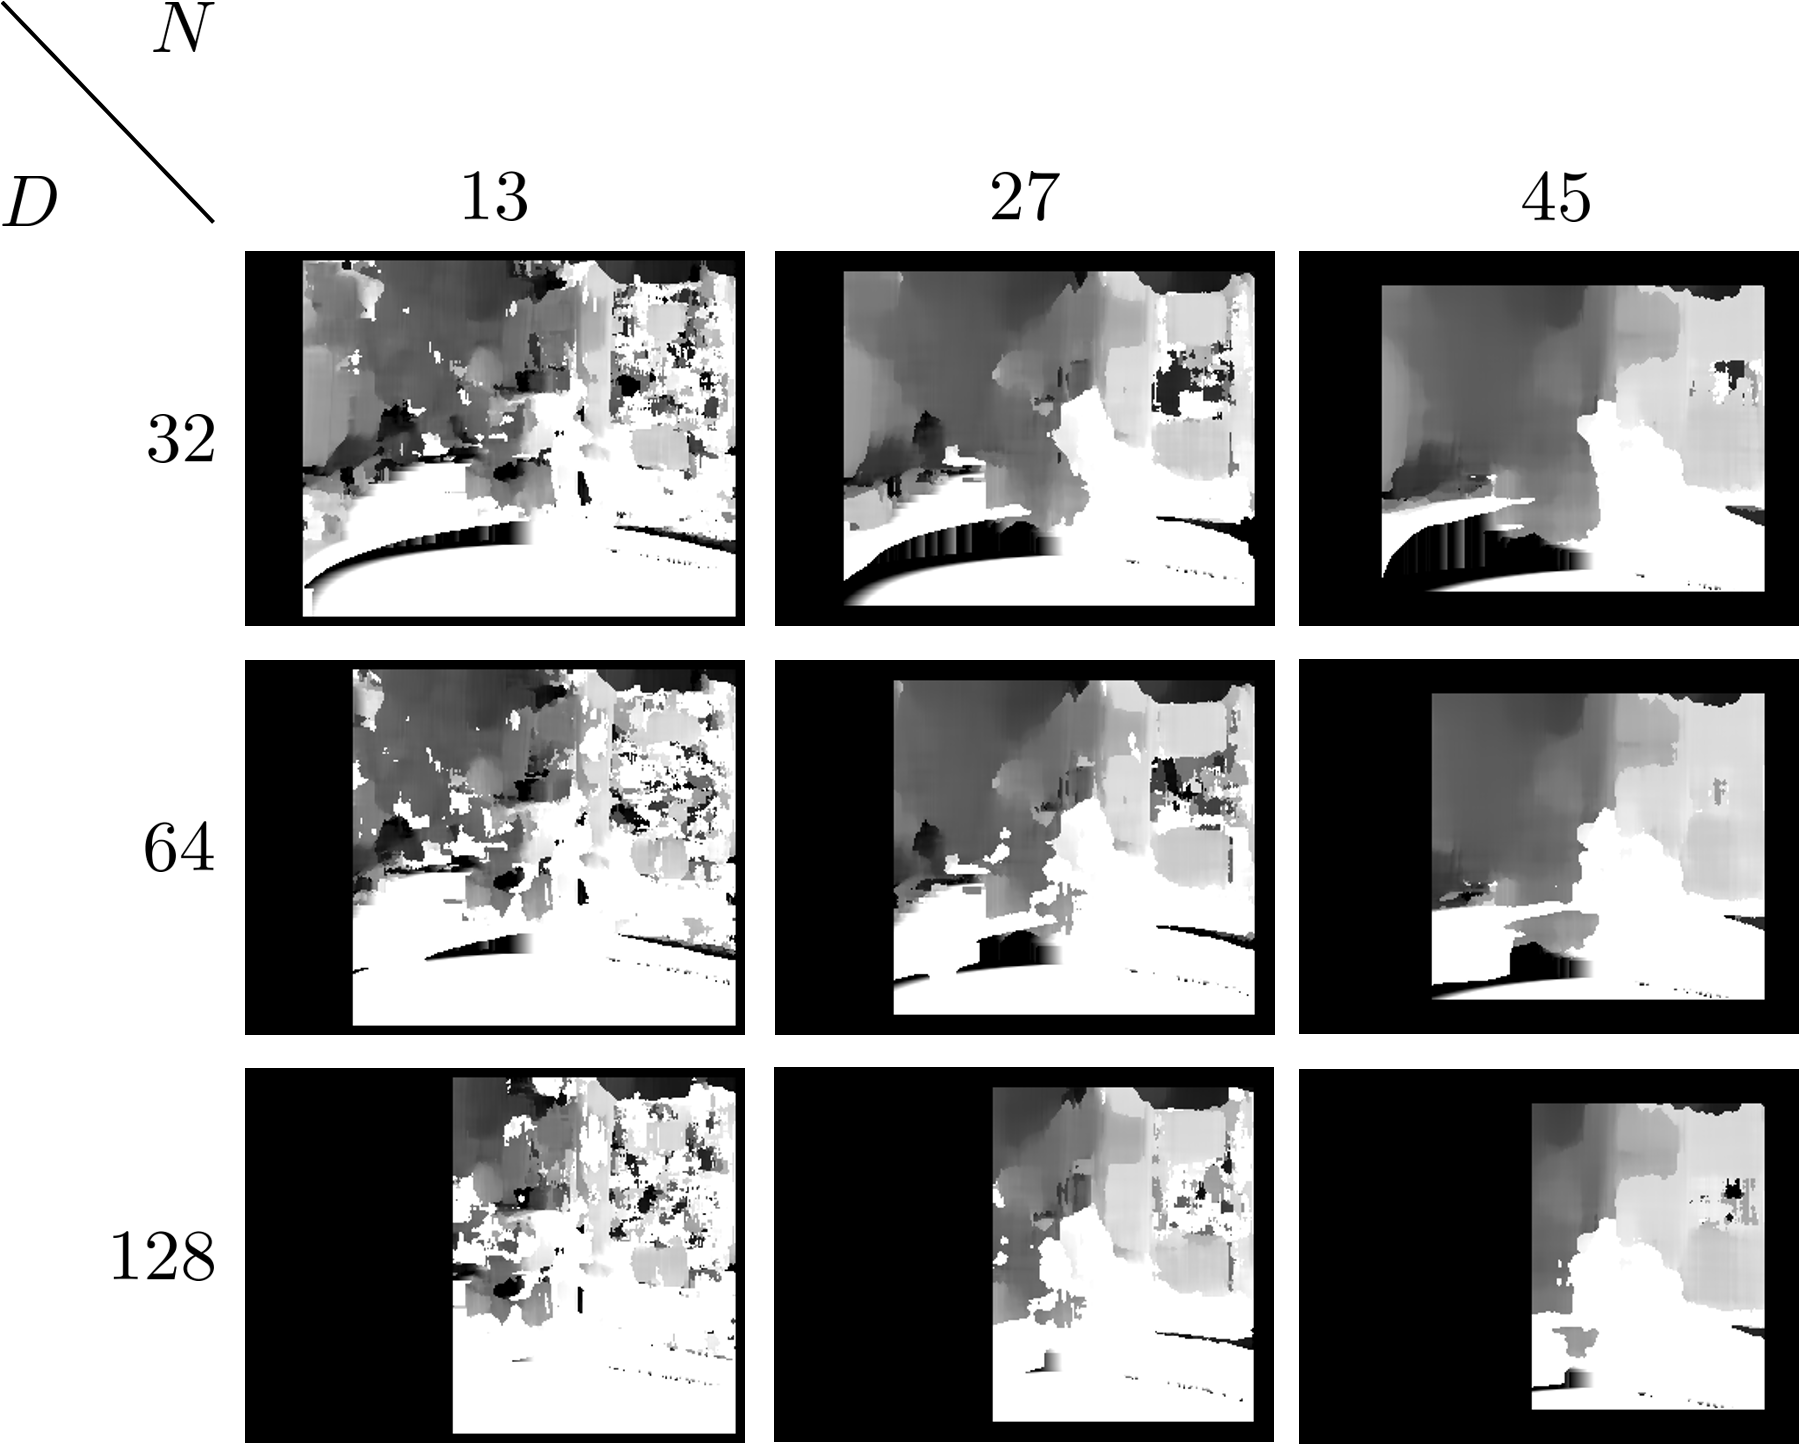
\includegraphics[scale=.2]{chapters/10_image_processing_experiments/img/disp_sad.png}}
	\subcaptionbox{Confidence weighted least squares disparity map. Please refer to figure \ref{fig::31_weighted_least_squares_disparity} and equation \ref{eq::31_wls_final} for the theory.}%
	[.45\linewidth]{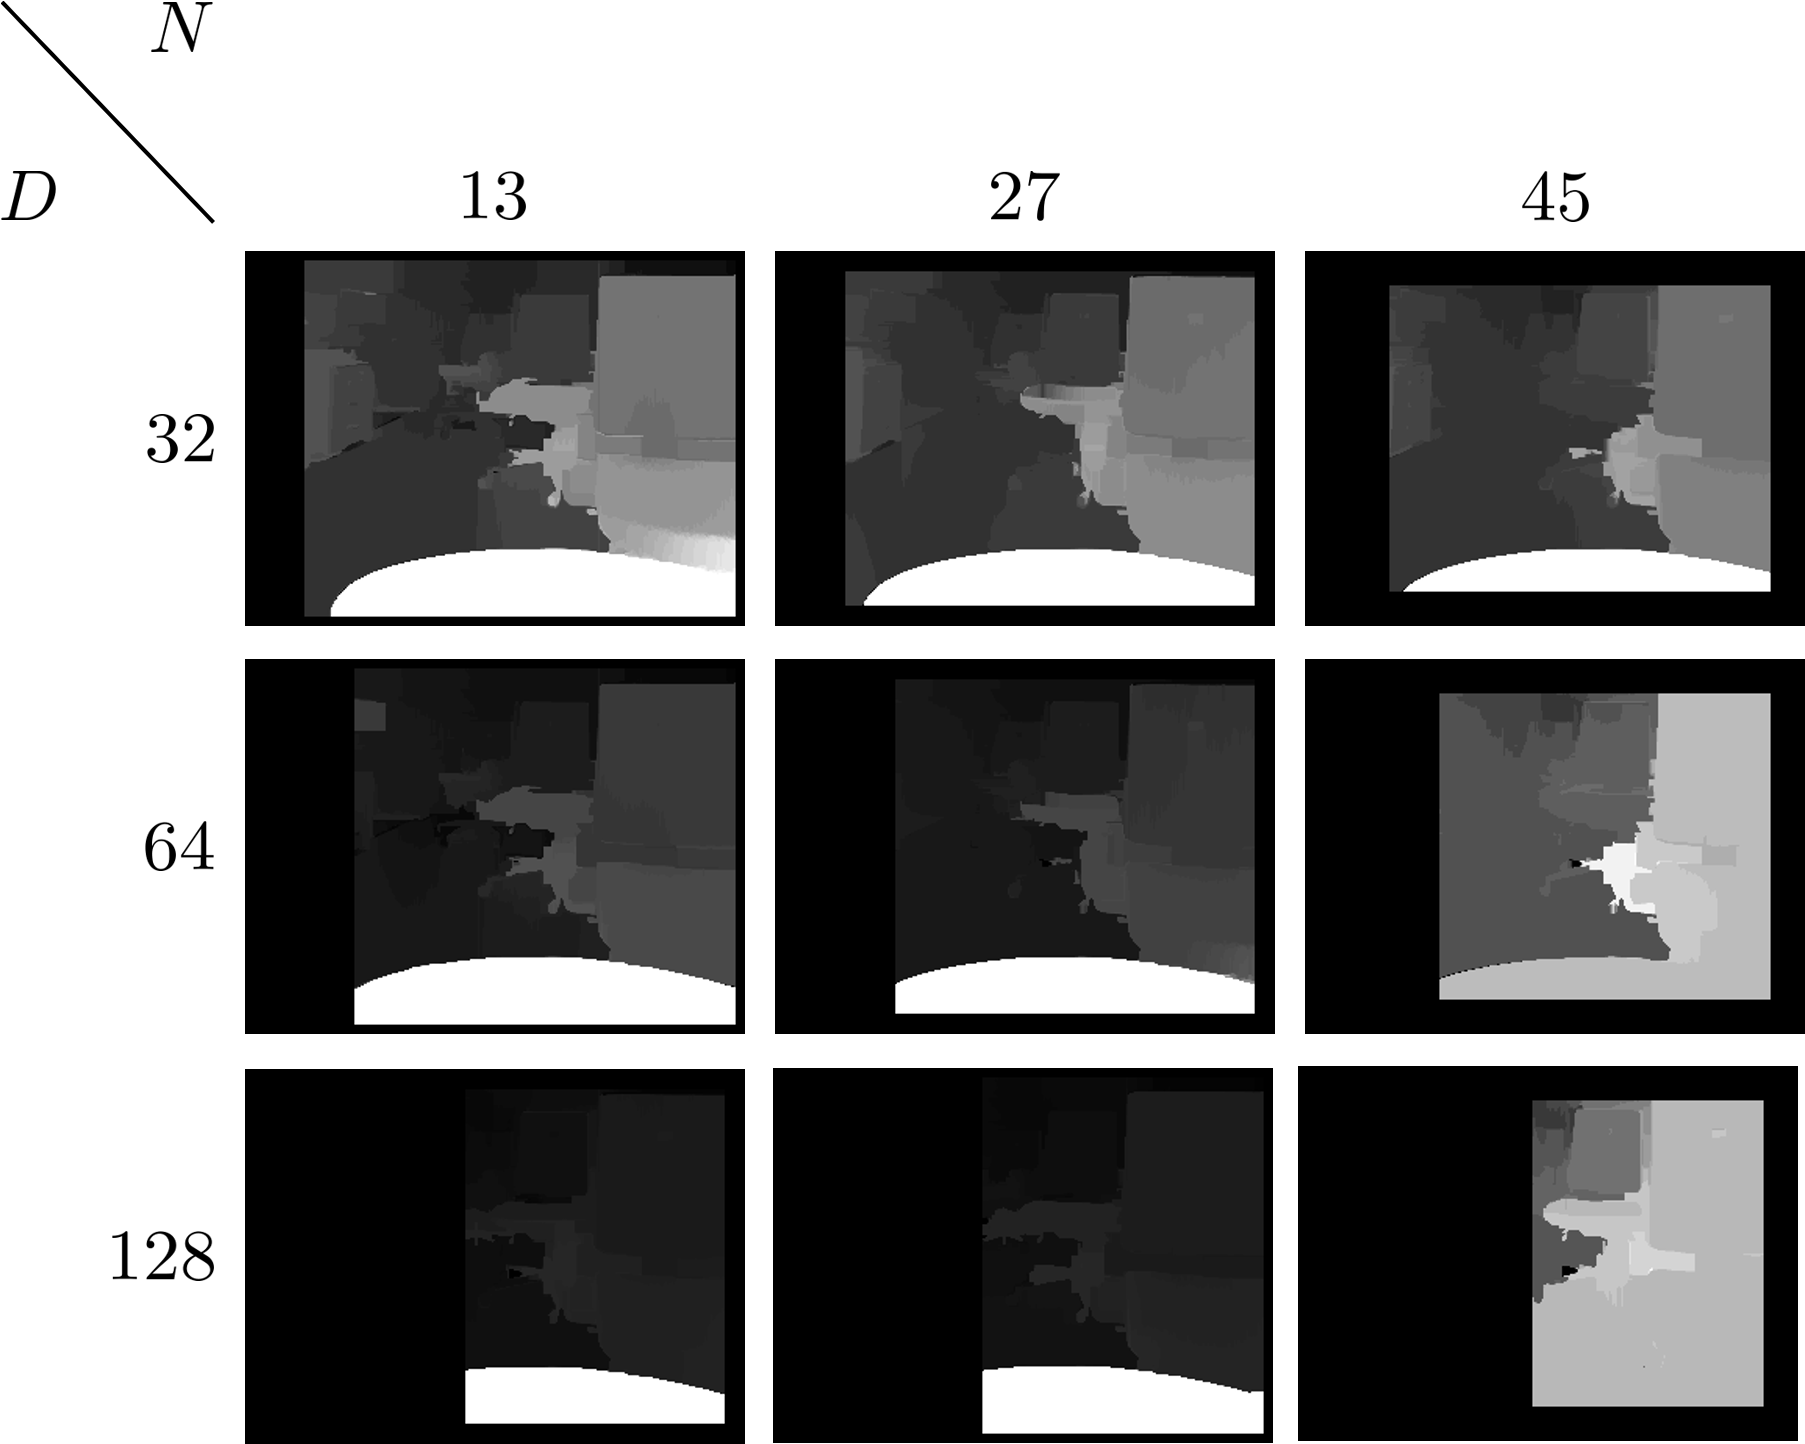
\includegraphics[scale=.2]{chapters/10_image_processing_experiments/img/disp_sad_wls.png}}
	\caption{Left disparity map and confidence weighted least squares disparity for changing SAD window sizes $N$ and number of disparities $D$.}
	\label{fig::102_disp}
\end{figure}
In combination with the confidence weighted least squares filtering, one can observe that most of the noise is already removed (figure \ref{fig::102_disp} (b)), for which it is more import to keep the information close to the images' borders. The number of disparities, was therefore chosen to be set to $D=32$, and the windows size to $N=13$ in the following. Within these depth maps, the global energy weighting $\lambda$ was set to $10^4$, and the local bilateral filter decay $\sigma$ to $1$, since the best performance was observed for them. The influence of those two parameters is visualized in figure \ref{fig::102_sigma_lambda}. It can be seen that, in good accordance with the theory, $\sigma$ contributes to the smoothing of the depth map, and that $\lambda$ enforces a change in depth across edges within the RGB images. Now given these parameters, the performance of the image processing pipeline was evaluated. It was run for $1000$ times and an average required time of $7.4\pm0.5\,\text{ms}$ on an Intel Core i7-7700HQ CPU at $2.8\,\text{GHz}$ was observed.
\begin{figure}[h!]
	\centering
	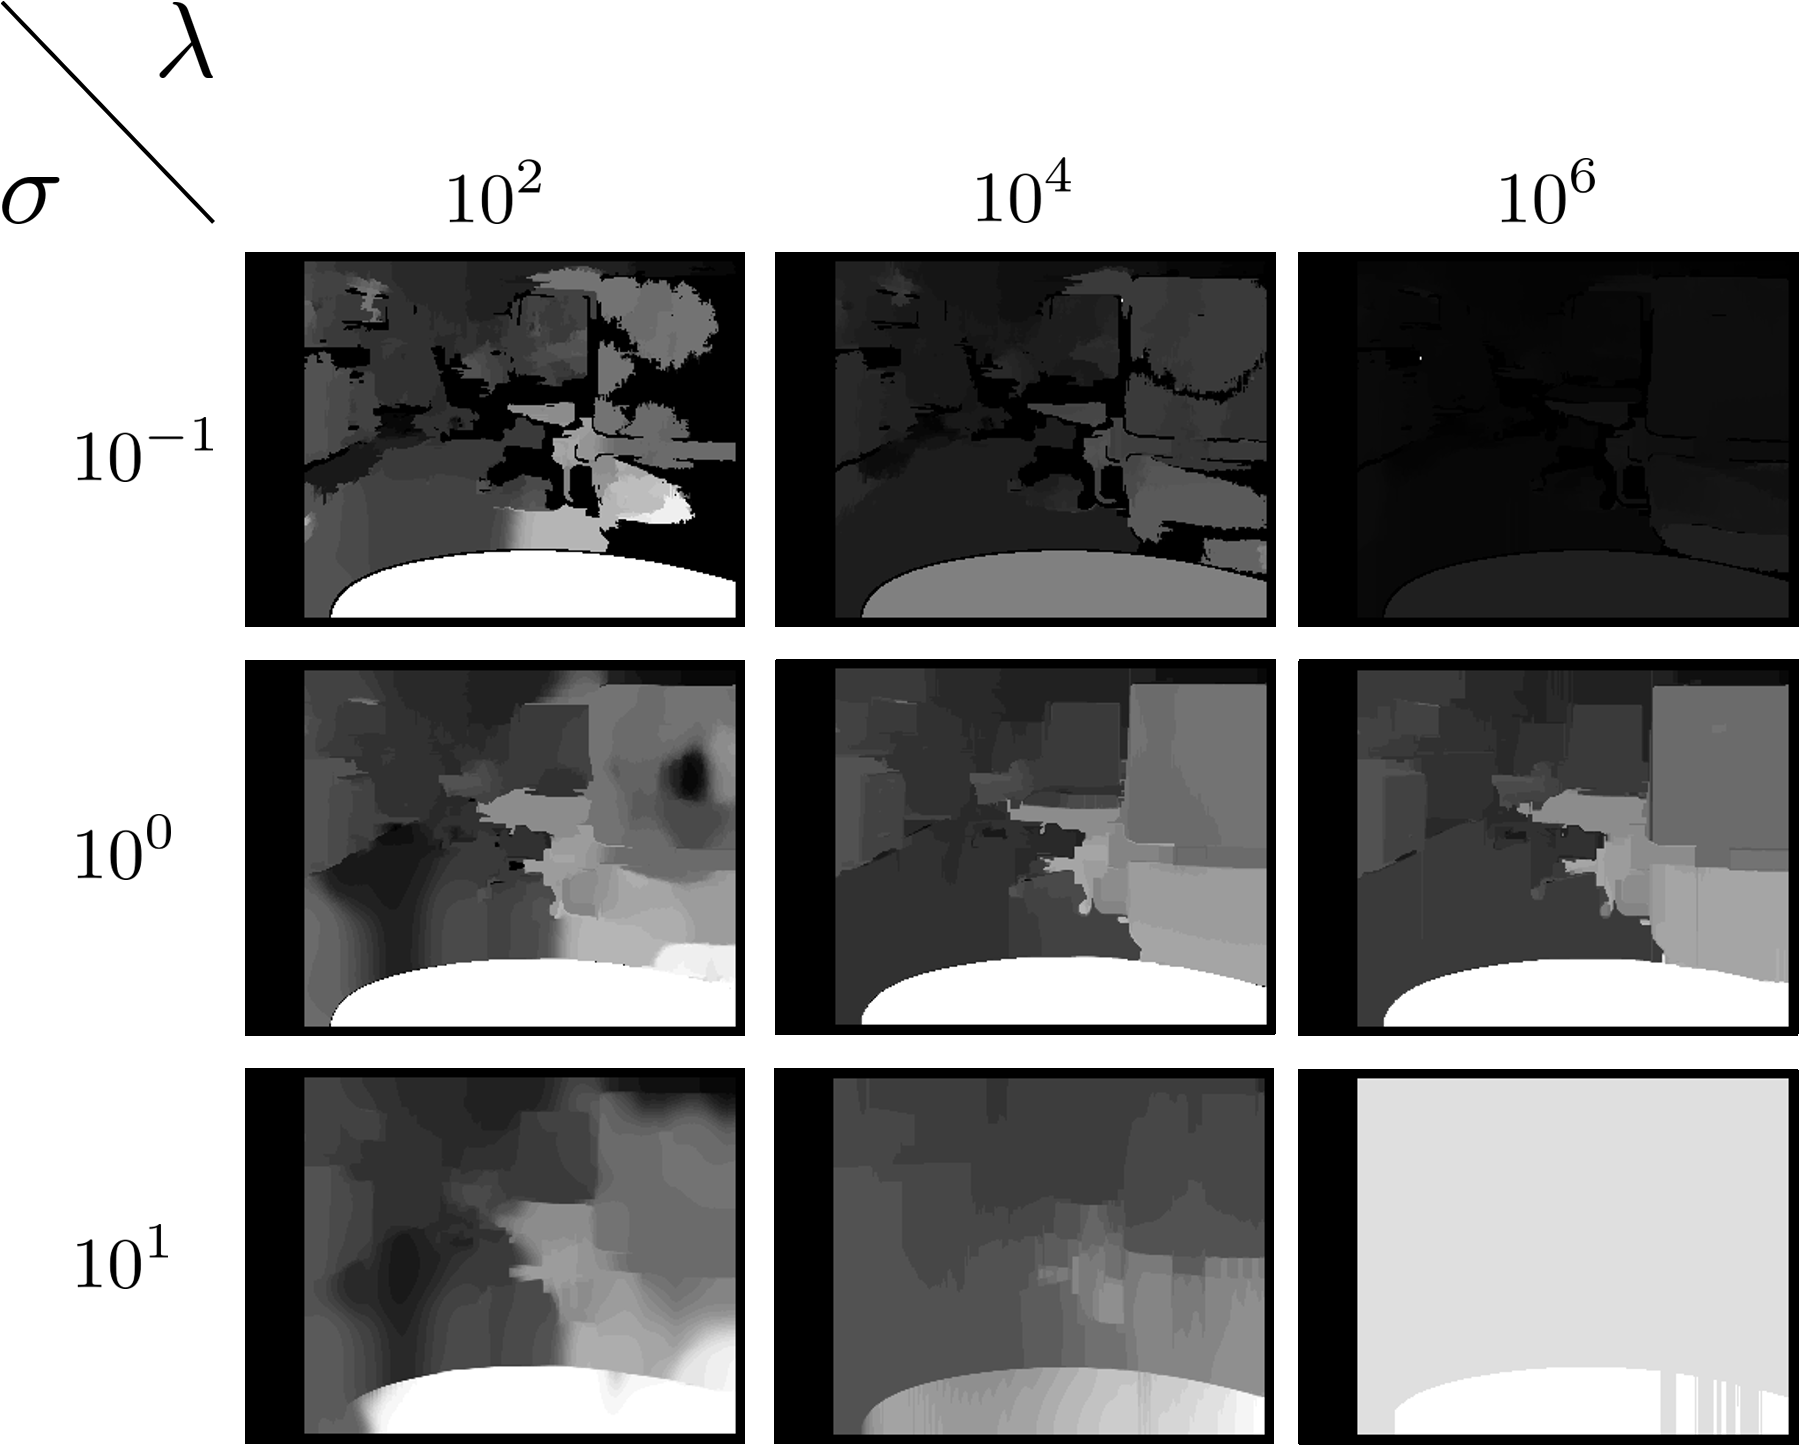
\includegraphics[scale=.2]{chapters/10_image_processing_experiments/img/sigma_lambda.png}
	\caption{Confidence weighted least squares disparity for changing energy weightings $\sigma$ and $\lambda$. Please refer to equations \ref{eq::31_weight} and \ref{eq::31_energy_function} for the theory.}
	\label{fig::102_sigma_lambda}
\end{figure}